 \chapter{Holographic Conformal Blocks} \label{ch:holographic}
 \subsection{Braney Motivation for AdS-CFT}
 During the Second Superstring Revolution, it was realised that String Theory was not just a theory of strings and that it included extended dynamical objects. In particular in the strong coupling limit, these objects could become much lighter than strings thus upset the presumed position of strings as fundamental objects. It was alos proposed that string theory itself is an effective theory. The 5 known string theories, type IA, type IIA, type IIB and heterotic SO(32) and $E_8 \times E_8$ were proposed to be limits of what was termed \emph{M-Theory}.
 
 
 These extended objects in string theory were termed \emph{branes}, as generalisations of membranes.
 In this section we present the stringy (and braney) arguments for the concrete example of the AdS/CFT correspondence proposed by Maldacena in his 1997 paper\cite{Maldacena:1}.
 
 \textbf{D-branes} in string theory are surfaces on which open strings with dirichlet boundary conditions can end. However, D-branes themselves are dynamical objects and may carry mass, charge, etc. 
 
 Starting with the superstring action:
 \begin{align}
  S=-\frac{1}{2\pi \alpha^\prime} \int \mathrm{d}^2\sigma \left\lbrace \partial_\alpha X_\mu \partial^\alpha X^\mu - i \bar{\psi}_\mu  \rho^\alpha \partial_\alpha \psi^\mu \right\rbrace
 \end{align}
  One may impose Raymond (R) or Neveu-Schwarz (NS) boundary conditions for the equation of motion of the fermionic string.
  \begin{align}
   \psi_\alpha^\mu(\sigma = 2\pi) &= \psi_\alpha^\mu(\sigma = 0)\;\;\;\,:\text{Raymond} \\
   \psi_\alpha^\mu(\sigma = 2\pi) &= -\psi_\alpha^\mu(\sigma = 0) \;:\text{Neveu-Schwarz}
  \end{align}

 \textbf{\emph{p}-branes} are supergravity solutions given by the metric:
 \begin{align}
  ds^2=H_p^{-1/2}(r) \left( -f(r)dt^2+\sum_{i=i}^p (dx^i)^2 \right) + H_p^{1/2}(r)\left(f^{-1}(r) dr^2 + r^2d\Omega_{n-p-2}^2 \right)
 \end{align}
 with
 \begin{align}
  f(r)=1-\left(\frac{r_0}{r}\right)^4 , \quad H_p(r)=1+\left( \frac{r_p}{r} \right)^{n-p-3}
 \end{align}


 
 \subsection{CFTs admitting a bulk dual}
 The Conformal field theories appearing in the AdS-CFT correspondence obey non-trivial conditions in addition to the usual consistency from crossing symmetry. It has been shown[insert ref. holography form CFT] that two necessary and sufficient condition for a CFT to admit a weakly coupled gravity dual are:
 \begin{enumerate}
  \item \emph{Have a large number of degrees of freedom, $N^2$}
  \item \emph{Have a finite number of low dimension operators}
 \end{enumerate}
  Although this has only been proven upto $\mathcal{O}(1/N)^2$ and for d=2 and d=4, it is conjectured that these conditions hold more generally. In particular, for theories with Einstein-like gravity duals, the low dimension operators are required to have spin $l \leq 2$ and their descendants since these correspond to spin $l$ particles in the bulk which are restricted upto spin 2 for the graviton mediating gravity.
  
  The operator spectrum may be divided into single trace and multi trace operators. Single trace operators correspond to single particle states adn multi trace operators correspond to multi particle states. The contact witten diagrams are represented by the infinite tower of multi trace operators. The exchange witten diagram corresponds to an exchage of single trace primary and an infite tower of multi trace operators. It will be helpful at this stahe to n;ote that the geodesic feynman diagram singles out the single trace primary exchange and calculates  it.
 \subsection{General Gauge-Gravity considerations}
 As intuitive and neat the braney ``derivation'' of the AdS-CFT correspondence is, in general one would like to have a non-stringy generalised criteria for when a CFT admits a gravity dual. To state this differently, how would a physicist with no knowledge of String theory ``discover'' the AdS-CFT correspondence [refer hartman et al]. This question has been asked 
  \section{AdS/CFT Considerations}
  Early on, from the work of Hawking and Bekenstein it was clear that the entropy of a region of spacce with a gravitational field was proportional to it's area and not its volume:
  \begin{align*}
   S=\frac{A}{4G}
  \end{align*}
  Where $G$ is newton's constant in $3+1$ Einstein's gravity. This led to the idea that in a theory with gravity, all the information about the theory in encoded on the boundary surface and not in the volume. This is in stark contrast to non-gravitational systems, say a volume of gas, where the entropy goes as the volume. This led to idea of the \emph{Holographic Principle} in the vein of encoding all the information from a 3-D object on a 2-D object.
  
  Very generally, the Anti-de-Sitter/Conformal Field Theory (AdS/CFT) correspondence is a conjectured duality between a full Quantum Gravity theory living in the bulk, and a Quantum Field Theory without gravity on the boundary. However, this full correspondence is quite difficult to test in its full form and commonly, the tests are performed in the semi-classical gravity limit of the correspondence which is made more concrete below. The necessary and sufficient condition for gravity to be weakly coupled is the presence of a large number of fields. This is imposed as the large $N$ limit. 
  
  If the bulk is to contain only spin 2 massless excitations, and not higher spins, the boundary theory must be strongly interacting. In order to have weak coupling in the bulk, large number of fields, in order to have einstein gravity in the bulk, strong coupling on the boundary.
  
  So we can assert that, in the CFT-AdS correspondence, the local operators in the boundary conformal field theory correspond to the quantum states on AdS d+1

  
  In its strongest form, the AdS/CFT correspondence predicts a duality between 10-dimensional type IIB string theory on the manifold $\text{AdS}_5 \times \text{S}^5$ (the ``bulk'') to $\mathcal{N}=4$ super yang mills theory with gauge group $U(N)$ on the boundary $S^4$ [check]. The duality holds when the following identifications are made:
  
  \begin{enumerate}
   \item $g_\text{YM}^2=4\pi g_\text{s}$ Here $g_\text{YM}$ is the coupling constant appearing in the Yang-Mills action.
   \item $\lambda \equiv g_\text{YM} N = \frac{R^4}{{\alpha^\prime}^2} $
   \item $\frac{\pi^4}{2N^2}=\frac{G_\text{N}}{R^8}$
  \end{enumerate}

  Consider gravity as a long distance effective theory with action:
  \begin{align*}
   \mathcal{S} = \frac{1}{G_N} \int \sqrt{g} (\mathcal{R} + \Lambda)
  \end{align*}
  Where $G_N \sim l_p^{D-2}$ where $l_p$ is the planck length and $G_N$ is the newtons constant in $D$ dimensions. This theory only makes sense when hte effective coupling of gravity $g_\text{eff}$ is small. 
  \begin{align*}
   g_\text{eff}^2 \sim \left( \frac{l_p}{L} \right)^{D-2} 
  \end{align*}
  Which physically means that we must restrict ourselves to modes of length scale $L >> l_p$ since at $L \sim l_p$ $g_\text{eff}$ becomes of order 1 and the theory doesn't make any sense.
  
  In this thesis, we will mainly be focussing on a weaker statement of the AdS/CFT conjecture. Namely, we shall be working in the  \emph{'t Hooft limit}: $N \rightarrow \infty$ 
  
  
  Now, in general, the prescription for calculating correlation functions is as follows:
  \begin{align*}
   \left\langle e^{\int \mathrm{d}^d x \mathcal{O}_i \phi_0 }\right\rangle = \mathcal{Z}_\text{grav} (\phi(x,z=0))
  \end{align*}
  
  Suppose we start with the correlator $\left\langle X \right\rangle$ where $X$ is some string of CFT operators. An \emph{operator insertion} of an operator $\mathcal{O}_i(x_i)$ at the point $x_i$ in the boundary theory corresponds to calculating the correlator.
  \begin{align*}
   \left\langle \mathcal{O}_i(x_i)X\right\rangle
  \end{align*}
  According to the prescription, the operator $\mathcal{O}_i$ is sourced by the boundary value $\phi_i(x)=\Phi_i(x,z=0)$ of a bulk field $\Phi(x,z)$ which in the (semi? check) classical limit extrimises the bulk action $\mathcal{S}_\text{grav}$. This means that exciting the mode $\Phi_i(x,z)$ in the bulk corresponds to adding the following term in the boundary action(and vice-versa):
  \begin{align*}
   \Delta\mathcal{S}= \int \mathrm{d}^dx \phi_i (x) \mathcal{O}_i(x)
  \end{align*}
  then the above mentioned correlator $\left\langle \mathcal{O}_i(x_i)X\right\rangle$ may be calculated (atleast formally) by the usual functional differentiation and setting the source to 0.
  \begin{align*}
   \left\langle \mathcal{O}_i(x_i)\mathcal{O}_1(x_1) \dots \mathcal{O}_n(x_n)\right\rangle = \left. \frac{\delta}{\phi_i(x_i)}\frac{\delta}{\phi_1(x_1)}\dots\frac{\delta}{\phi_n(x_n)} \mathcal{S}_\text{grav}(\Phi_i,\Phi_1\dots\Phi_n) \right|_{\phi_0=0,\phi_1=0\dots\phi_n=0}
  \end{align*}


  
  \begin{align*}
   \int \mathrm{d}^dx j(x) \mathcal{O}(x)
  \end{align*}
  to the action of the boundary theory. This operator insertion is sourced by the classical source $j(x)$ and the generating functional of connected correlators is given by:
  \begin{align*}
   W[j] = -\ln \left\langle e^{\int \mathrm{d}^d x \mathcal{O}_i \phi_0 }\right\rangle
  \end{align*}
  
  In general, starting from operator insertions $\mathcal{O}_1(x_1), \mathcal{O}_2(x_2), \mathcal{O}_3(x_3), \mathcal{O}_4(x_4)$ at the boundary, and assuming only cubic interactions in the bulk, the \emph{full} 4-point correlator is given by the bulk object ($\mathcal{K}(x,y)$ represents the bulk to boundary propagator from a bulk point $x$ to a boundary point $y$ and $\mathcal{G}(x,y)$ represents the bulk to bulk propagator between two bulk points $x$ and $y$):
  
  \begin{align*}
   \left\langle \mathcal{O}_1(x_1) \mathcal{O}_2(x_2) \mathcal{O}_3(x_3) \mathcal{O}_4(x_4)\right\rangle = \\   
   \int_{\forall AdS} \mathrm{d}^{d+1}x \int_{\forall AdS} \mathrm{d}^{d+1}y \mathcal{K}(x,x_1)\mathcal{K}(x,x_2) \mathcal{G}(x,y) \mathcal{K}(y,x_3) \mathcal{K}(y,x_4)
  \end{align*}
  This interaction is represented by the Witten diagram

   Now the proposal of Kraus, Hijano et al is as follows: The bulk object computing the conformal partial wave is the geodesic Witten Diagram. 
   \subsection{Explicit Computation of the Geodesic Witten Diagram}
   Consider the following geodesic witten diagram:
   \begin{align}
    W_{\Delta,0}(x_i)=\int_{\gamma_{12}} \mathrm{d}\lambda^\prime \int_{\gamma_{34}} \mathrm{d}\lambda \mathcal{K}(y(\lambda),x_1) \mathcal{K}(y(\lambda),x_2) \mathcal{G}(y(\lambda),y(\lambda^\prime);\Delta)\mathcal{K}(y(\lambda^\prime),x_3) \mathcal{K}(y(\lambda^\prime),x_4) \label{eqw}
   \end{align}
  Define $\phi_{\Delta}^{12}(y(\lambda^\prime))$ to be the part of $W$ that depends only on the geodesic $\gamma_{12}$: 
  \begin{align}
   \phi_{\Delta}^{12}(y(\lambda^\prime))\equiv  \int_{\gamma_{12}} \mathcal{K}(y(\lambda),x_1) \mathcal{K}(y(\lambda),x_2) \mathcal{G}(y(\lambda),y(\lambda^\prime);\Delta) \label{eqphi}
  \end{align}
  Since$\mathcal{G}$ is the green's function for the Klein-Gordon equation in AdS space, it is clear from the form of $\phi_{\Delta}^{12}(y(\lambda^\prime))$ as a convolution of the green's function and some function that it is a normalisable solution of the inhomogenous Klein-Gordon equation with the source term.
  \begin{align*}
   \mathcal{J}=(\nabla^2(y)-m^2)\phi_{\Delta}^{12} = \delta(y) %!!!CHECKA!!!
  \end{align*}
  Check Appendix [] for a derivation of the propagators $\mathcal{G}$ and $\mathcal{K}$. These are given by:
  
  Since the correlation functions satisfy
  \begin{align*}
   \left\langle \phi_1(x_1) \phi_2(x_2) \dots \phi_n(x_n) \right\rangle = \left| \frac{\partial x^\prime}{\partial x}\right|_{x=x_1}^{\Delta_1/d} \cdots \left| \frac{\partial x^\prime}{\partial x}\right|_{x=x_n}^{\Delta_n/d} \left\langle \phi_1(x_1^\prime) \phi_2(x_2^\prime) \dots \phi_n(x_n^\prime) \right\rangle
  \end{align*}
  
  In general, the 4 point functions depend on the conformally invariant cross ratios $u,v$
  
  \begin{align}
   u=\frac{|x_1-x_2||x_3-x_4|}{|x_1-x_3||x_2-x_4|}, \;\;\; v = \frac{|x_1-x_2||x_3-x_4|}{|x_2-x_3||x_4-x_1|}
  \end{align}

   For computational convenience, we use conformal symmetry to send 3 of the 4 points in the 4-point correlator $x_1, x_2$ and $x_4$ to $\infty$, 0 and 1 respectively. The correlator and the conformal partial wave [check] remain invariant under this $SO(d+1,1)$ transformation.
   
  i.e. upto some overall factor we can equivalently calculate the quantity 
  \begin{align*}
  W_{\Delta,0}(u,v)= \left\langle \mathcal{O}_1(\infty) \mathcal{O}_2(0) P_{\Delta,0} \mathcal{O}_3(1-z) \mathcal{O}_4(1)\right\rangle \label{partialwave}
  \end{align*}
 
  \begin{multline}
  W_{\Delta,0}(u,v) = \lim_{x_1 \to \infty} |x_1|^{2\Delta_1} \frac{1}{C_{12\mathcal{O}}C_{34}^{\mathcal{O}}} \left\langle \mathcal{O}_1(x_1) \mathcal{O}_2(0) P_{\Delta,0} \mathcal{O}_3(1-z) \mathcal{O}_4(1)\right\rangle \\ = \lim_{x_1 \to \infty} |x_1|^{2\Delta_1}  \frac{1}{{x_{1}^2}^{\frac{1}{2}(\Delta_1+\Delta_2)}{(x_{3}-1)^2}^{\frac{1}{2}(\Delta_3+\Delta_4)}} \left(\frac{(x_{1}-1)^2} {(x_{1}-1+z)^2}\right)^\frac{\Delta_{34}}{2} \left(\frac{(-1)^2}{(x_{1}-1)^2}\right)^\frac{\Delta_{12}}{2} G_{\Delta,0}(u,v) \\ = u^{-\frac{(\Delta_3+\Delta_4)}{2}} G_{\Delta,0}(u,v)
  \end{multline}
 
  Since in radial quantisation a CFT on the euclidean plane $\mathbb{R}^d$ is identified with the CFT on the cylinder $\mathbb{R}\times \mathbb{S}^{d-1}$, which is exactly the conformal boundary of $AdS_{d+1}$. Under the above transfrmations, the $x_1 - x_2$ geodesic $\gamma_{12}$ becomes the geodesic $\rho=0$ in global AdS coordinates because taking $x_1 \to \infty, x_2 \to 0$ corresponds on the cylinder to taking $t_1 \to \infty, t_2 \to -\infty$ [INCLUDE FIGURE]. This imposes additional rotational symmetry on the AdS Klein-Gordon solution $\phi_{12}^\Delta$. We will solve the KG equation in global AdS coordinates:
  
  
  \begin{figure}[!h]
\centering
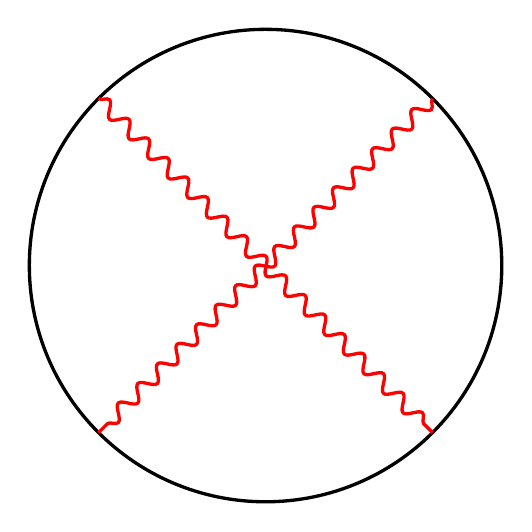
\begin{tikzpicture}[scale=2,>=stealth]
%Draw Circle radius 1 cm
  \def\radi{1.5cm}
    \draw[black,very thick] (0,0) circle (\radi);
   % \foreach \angle/\count in {45/1,135/2,225/3,315/4}
    %    {
        
\tikzset{snake it/.style={decorate, decoration=snake}}
%Draws the 3 acceleration vectors directed inward and offset slightly from the distance vectors
       % \draw [name=acceleration vectors,very thick, snake it]
        %    (\angle:1.2cm) -- node[midway] {} (\angle:0.9cm) ;
         %     \path [draw=blue,snake it](-4,0) -- (-2,0) -- (2,0) -- (4,0);
  %\draw[draw=blue, snake it] (2,0) arc (0:180:2cm);
   % } snake it
    
        \path[coordinate] (0,0)  coordinate(A)++( 45:\radi) coordinate(B1);
        \path[coordinate] (0,0)  coordinate(A)++( 135:\radi) coordinate(B2);
        \path[coordinate] (0,0)  coordinate(A)++( -45:\radi) coordinate(B3);
        \path[coordinate] (0,0)  coordinate(A)++( -135:\radi) coordinate(B4);
        \draw[draw=red, snake it, very thick] (B1)--(B4);
        \draw[draw=red, snake it, very thick] (B2)--(B3);
\end{tikzpicture}
\end{figure}
 \begin{align*}
  ds^2=\frac{1}{\cos^2\rho} \left( d \rho^2 + dt^2 + \sin^2 \rho \Omega^2_{d-1} \right)
 \end{align*}
  The K-G equation in global coordinates is given by (where $m^2=\Delta(\Delta-d)$):
  \begin{align}
   \left( \cos^2 \rho \partial^2_\rho + (d-1)\cot \rho \partial_\rho + \cos^2 \rho \partial^2_t -m^2 \right) \phi^{12}_{\Delta}(y) = 0 \label{KGglob}
  \end{align}
  Now, the time dependence of $\phi$ may be calculated by considering the product of two bulk-to-boundary propagators on a fixed time $t$ slice:
  \begin{align*}
   \mathcal{K}(t,t_1) \mathcal{K}(t,t_2) \propto e^{-\Delta_{12}t}
  \end{align*}
  plugging this into eqn. \ref{KGglob} gives
  \begin{align}
   \left( \cos^2 \rho \partial^2_\rho + (d-1)\cot \rho \partial_\rho + \cos^2 \rho \Delta_{12}^2 -m^2 \right) \phi^{12}_{\Delta}(y) = 0 \label{KGglob1}
  \end{align}
  
  This differential equation can be converted into the hypergeometric equation with the correct choice of substituitions. Changing the variables from $\rho \to \eta$ with the substituition $\eta = \cos ^2 \rho$ gives:
  \begin{align}
   \left( 2 \eta (\eta-1)  \partial_\eta^2 + (d-2+2 \eta) \partial_\eta + \frac{\eta \Delta_{12}^2 - \Delta(\Delta-d) }{2\eta} \right) \phi = 0
  \end{align}
  The further substitution $\phi(\eta) = \eta^{\Delta/2} f(\eta)$ (or $\phi(\eta) = \eta^{(d-\Delta)/2} f(\eta)$) reduces the equation to a hypergeometric equation:
    \begin{align}
   \left[ \eta (1-\eta)  \partial_\eta^2 + \left(-\frac{d}{2}+1+\Delta -(1+\Delta)\eta\right) \partial_\eta - \frac{\Delta^2-\Delta_{12}^2}{4} \right] f(\eta) = 0
  \end{align}
  This has the same form as the hypergeometric differential equation
  
  \begin{align}
   z(1-z)\frac{d^2 w}{dz^2} + (c-(1+a+b)z)\frac{dw}{dz}-abw =0
  \end{align}
  for
  \begin{align}
   a &= \frac{\Delta-\Delta_{12}}{2} \\
   b &= \frac{\Delta+\Delta_{12}}{2} \\
   c &= -\frac{d}{2}+\Delta +1
  \end{align}
  Which gives the solution
  \begin{align}
   f(\eta) &= {}_2 F_1 \left(\frac{\Delta-\Delta_{12}}{2},\frac{\Delta+\Delta_{12}}{2},-\frac{d}{2}+\Delta +1; \eta \right) \\   
   \implies \phi^{12}_{\Delta}(\rho) &=  {}_2 F_1 \left(\frac{\Delta-\Delta_{12}}{2},\frac{\Delta+\Delta_{12}}{2} ,  -\frac{d}{2}+\Delta +1 ; \cos^2 \rho \right) \cos^\Delta \rho 
  \end{align}
  Then the full solution including time dependence is given by
 \begin{multline}
   \phi^{12}_{\Delta}(\rho, t) = \beta_{\Delta 1 2 } e^{\Delta_1 t_1 - \Delta_2 t_2}\times e^{-\Delta_{12}t} \\ \times {}_2 F_1 \left(\frac{\Delta-\Delta_{12}}{2},\frac{\Delta+\Delta_{12}}{2} ,  -\frac{d}{2}+\Delta +1 ; \cos^2 \rho \right) \cos^\Delta \rho
 \end{multline}
  Now, as we see from \ref{eqw} and \ref{eqphi} we need to evaluate $\phi^{12}_{\Delta}(\rho, t)$ on the geodesic $\gamma_{34}$. This is most conveniently done in Poincar\'{e} coordinates since in Poincar\'{e} AdS$_3$ the geodesics are just semi-circles. However, the transformation properties of the function $\phi^{12}_{\Delta}$ are not trivial when moving from global to Poincar\'{e} coordinates. The bulk-bulk propagator $\mathcal{G}$ is a function of only the geodesic distance between the two boundary points, therefore independent of the 
  
  However, the bulk-to-boundary propagator is a solution of the homogenous AdS wave equation which diverges in a prescribed manner in the bulk.
  
  \begin{align}
   (\Box - m^2) \mathcal{K} = 0
  \end{align}
In Poincar\'{e} coordinates, the $u \to 0$ behavior of $\mathcal{K}$ is 
\begin{align}
 \lim_{u \to 0} \mathcal{K}_{Poincar\'{e}}(u,x;x^\prime) \to u^{\Delta_-}\delta(x-x^\prime)
\end{align}
This is because the non-renormalizable bulk modes of the AdS wave equation in Poincar\'{e} coordinates behave as $u^{\Delta_-}$ near the boundary and therefore $\mathcal{K}$ should reproduce that behavior when a source function on the boundary sources a bulk field.

However, the non-renormalizable bulk modes of the AdS wave equation in global coordinates behave as $\cos^{\Delta_-} \rho$ near the boundary. So 
\begin{align}
 \lim_{\rho \to \pi/2} \mathcal{K}_{global}(\rho,t,\Omega;t^\prime, \Omega^\prime) \to \cos^{\Delta_-}\rho \delta(x-x^\prime)
\end{align}
  check McGreevy http://physics.ucsd.edu/~mcgreevy/fall08/handouts/lecture14.pdf 
  
  The map from global coordinates $(\rho, t)$ to Ponicar\'{e} coordinates $u,x^i$ is given by
  \begin{align}
   e^{-2t} = u^2 + |x|^2, \;\;\;\; \cos^2\rho = \frac{u^2}{u^2 + |x|^2} \label{globaltopoincare}
  \end{align}

  Hence, the global and poincare bulk-to-boundary propagators differ by a factor of $|x_i|^{\Delta_i}$. Stripping these factors off, for the sake of convinience gives the function $\phi^{12}_{\Delta}$ in Poincare coordinates
   \begin{multline}
   \phi^{12}_{\Delta}(u,x^i) = \beta_{\Delta 1 2 } e^{\Delta_1 t_1 - \Delta_2 t_2}\times e^{-\Delta_{12}t} \\ \times {}_2 F_1 \left(\frac{\Delta-\Delta_{12}}{2},\frac{\Delta+\Delta_{12}}{2} ,  -\frac{d}{2}+\Delta +1 ; \cos^2 \rho \right) \cos^\Delta \rho \label{phipoincare}
 \end{multline}
 Where now the global coordinates $(\rho,t)$ on the right hand side of \ref{phipoincare} are to be viewed as functions of the Poincar\'{e} coordinates by \ref{globaltopoincare}. 
 
 Geodesics in AdS$_3$ are semi-circles, see appendex entry \ref{adsgeodesic}  for a derivation, and with the particular choice of coordinates in \ref{partialwave} the geodesic $\gamma_{34}$ connecting points $z_3 = 1-z$ and $z_4 = 1$ lies exactly in an AdS$_3$ slice of AdS$_{d+1}$. Therefore the equation of $\gamma_{34}$ can be written as 
 \begin{align}
  u^2 + 
 \end{align}

  \section{Mellin Space Representations of CFT Correlators}
  \subsection{Single Trace, double trace operators and shadow operators, conglomeration of operators}
  See fitzpatrick, kaplan, Unitarity and the Holographic S matrix
  \section{Monodromy Method}
  \section{Embedding Formalism and The Conformal Casimir}
